\documentclass[12pt]{article}

\usepackage{sbc-template}
\usepackage{graphicx,url}
\usepackage[utf8]{inputenc}
\usepackage[brazil]{babel}
  \usepackage{booktabs} 

     
\sloppy

\title{ESP32-LLM: Uma Avaliação Experimental da Confiabilidade de Código Gerado por Large Language Models para Sistemas Embarcados}

\author{Renato William Rodrigues de Souza}

\address{Instituto Federal do Sudeste de Minas Gerais (IF Sudeste MG)\\
	Campus Manhuaçu -- Pós-Graduação Lato Sensu em Desenvolvimento Full Stack\\
	Manhuaçu -- MG -- Brasil
}
\begin{document} 

\maketitle

\begin{abstract}
This study evaluates the reliability of ESP32 code generated by three Large Language Models (LLMs) across different levels of task difficulty. A benchmark composed of 30 tasks derived from a real embedded-system firmware was defined, with 10 easy, 10 medium, and 10 hard tasks. The same standardized prompts were submitted to GPT-5.6-Sol, DeepSeek-V4-Pro, and Claude-Sonnet-5, resulting in 90 generated solutions. The evaluation combined compilation, automated functional tests, qualitative assessment, and statistical analysis. The results indicate high performance on easy and medium tasks, while a marked degradation was observed on hard tasks. No statistically significant differences were found among the models regarding compilation or overall functional performance, whereas task difficulty had a significant effect for all three LLMs. The findings also show that highly rated qualitative solutions may still fail to compile or integrate correctly in the target firmware.
\end{abstract}
     
\begin{resumo}
Este trabalho avalia a qualidade de código ESP32 gerado por três Large Language Models (LLMs) em diferentes níveis de dificuldade. Foi definido um benchmark composto por 30 tarefas derivadas de um firmware real de sistema embarcado, sendo 10 fáceis, 10 médias e 10 difíceis. Os mesmos prompts padronizados foram submetidos ao GPT-5.6-Sol, DeepSeek-V4-Pro e Claude-Sonnet-5, totalizando 90 soluções geradas. A avaliação combinou compilação, testes funcionais automatizados, análise qualitativa e análise estatística. Os resultados indicaram elevado desempenho nas tarefas fáceis e médias, mas forte queda nas tarefas difíceis. Não foram observadas diferenças estatisticamente significativas entre os modelos quanto à compilação ou ao desempenho funcional global, enquanto o nível de dificuldade apresentou efeito significativo para as três LLMs. Os resultados também mostram que soluções qualitativamente bem avaliadas podem ainda falhar na compilação ou na integração com o firmware alvo.
\end{resumo}

\section{Introdução}
\label{sec:introducao}

Large Language Models (LLMs) têm sido amplamente utilizados em atividades de Engenharia de Software, incluindo geração, completação e transformação de código. Benchmarks como HumanEval e MBPP consolidaram testes funcionais como uma das principais formas de avaliar a correção das soluções geradas~\cite{chen2021codex,austin2021program}. Entretanto, tarefas algorítmicas autocontidas não representam integralmente as condições do desenvolvimento de sistemas embarcados, nos quais o código pode depender de bibliotecas, APIs de hardware, estado compartilhado e contratos de integração com o firmware~\cite{englhardt2023embedded}.

Nesse contexto, uma solução aparentemente correta quando analisada isoladamente pode falhar durante a compilação, execução ou integração no sistema-alvo. Estudos recentes indicam que a complexidade das tarefas influencia o desempenho de LLMs em programação de sistemas baseados em microcontroladores~\cite{babiuch2026benchmarking}, reforçando a necessidade de avaliações que combinem diferentes dimensões da qualidade e considerem o contexto real de execução.

Este trabalho apresenta o \textit{ESP32-LLM Benchmark}, um estudo experimental para avaliar a confiabilidade de código ESP32 gerado por LLMs. Neste estudo, confiabilidade é operacionalizada como a capacidade de a solução gerada compilar, satisfazer testes funcionais previamente definidos e preservar os contratos necessários à integração com o firmware-alvo. O benchmark compreende 30 tarefas derivadas de um firmware real e distribuídas igualmente entre três níveis de dificuldade. Três LLMs foram submetidas aos mesmos prompts, sem ciclos de correção ou refinamento, produzindo 90 soluções para avaliação.

O estudo é orientado pelas seguintes questões de pesquisa: \textbf{RQ1}: Como as LLMs avaliadas diferem quanto à capacidade de gerar código ESP32 compilável e funcionalmente correto? \textbf{RQ2}: Em que medida o nível de dificuldade das tarefas afeta a correção funcional do código ESP32 gerado pelas LLMs? \textbf{RQ3}: Em que medida avaliações qualitativas do código gerado estão associadas ao seu desempenho objetivo de compilação e testes funcionais? \textbf{RQ4}: Quais são os principais tipos de falha encontrados nas soluções geradas para tarefas de maior dificuldade?

As principais contribuições deste trabalho são: (i) um benchmark com 30 tarefas derivadas de um firmware ESP32 real e organizadas em três níveis de dificuldade; (ii) a avaliação experimental de 90 soluções produzidas por três LLMs sob um protocolo padronizado; (iii) a combinação de compilação, testes funcionais e avaliação qualitativa cruzada; e (iv) a análise do efeito da dificuldade, da relação entre avaliação qualitativa e desempenho objetivo e das falhas observadas nas tarefas de maior complexidade.


\section{Fundamentação e Trabalhos Relacionados}
\label{sec:relacionados}

Benchmarks como HumanEval~\cite{chen2021codex} e MBPP~\cite{austin2021program} consolidaram o uso de testes funcionais como evidência objetiva da correção de código gerado por LLMs. Entretanto, avaliações recentes indicam que a qualidade dessas soluções envolve múltiplas dimensões além da aprovação em testes~\cite{umama2025slr,nogueira2026probe,patcas2026quality}. Em sistemas embarcados, essa questão é particularmente relevante devido às dependências de hardware, bibliotecas, APIs e estado compartilhado do firmware.

No contexto de sistemas embarcados, Babiuch e Smutny~\cite{babiuch2026benchmarking} avaliaram LLMs em aplicações baseadas em microcontroladores, incluindo ESP32, e observaram influência da complexidade das tarefas sobre o desempenho. Esses resultados reforçam a necessidade de considerar não apenas a lógica local das soluções, mas também sua capacidade de integração com o sistema-alvo. A Tabela~\ref{tab:related_work_comparison} compara as principais características das abordagens discutidas.

\begin{table*}[ht]
\centering
\caption{Comparação de abordagens para avaliação de código gerado por LLMs.}
\label{tab:related_work_comparison}
\resizebox{\textwidth}{!}{%
\begin{tabular}{@{}lcccccc@{}}
\toprule
\textbf{Trabalho} &
\textbf{Tarefas reais} &
\textbf{Contexto de firmware} &
\textbf{Compilação} &
\textbf{Testes funcionais} &
\textbf{Avaliação qualitativa} &
\textbf{Análise de falhas} \\
\midrule
HumanEval~\cite{chen2021codex} & Não & Não & -- & Sim & Não & Não \\
MBPP~\cite{austin2021program} & Não & Não & -- & Sim & Não & Não \\
\cite{umama2025slr} & -- & -- & -- & -- & -- & -- \\
PROBE~\cite{nogueira2026probe} & -- & Não & -- & -- & Sim & -- \\
\cite{patcas2026quality} & -- & Não & -- & -- & Sim & Sim \\
\cite{babiuch2026benchmarking} & -- & Sim & Sim & Sim & -- & -- \\
\textbf{Este trabalho} & \textbf{Sim} & \textbf{Sim} & \textbf{Sim} &
\textbf{Sim} & \textbf{Sim} & \textbf{Sim} \\
\bottomrule
\end{tabular}%
}
\end{table*}

Diferentemente dos benchmarks baseados predominantemente em problemas autocontidos, este trabalho utiliza 30 tarefas derivadas de um mesmo firmware ESP32 real e organizadas por diferentes graus de dependência contextual. O protocolo combina compilação e integração no ambiente-alvo, 151 casos de teste funcionais, avaliação qualitativa cruzada e análise das causas de falha nas tarefas difíceis, permitindo examinar conjuntamente a correção executável e a compatibilidade das soluções com o contexto do firmware.

\section{Metodologia}
\label{sec:metodologia}
A Figura~\ref{fig:fluxo-metodologico} sintetiza o desenho experimental, desde a derivação das tarefas do firmware de referência até a geração das soluções, avaliação objetiva, avaliação qualitativa cruzada e análise estatística.

\begin{figure}[ht]
    \centering
    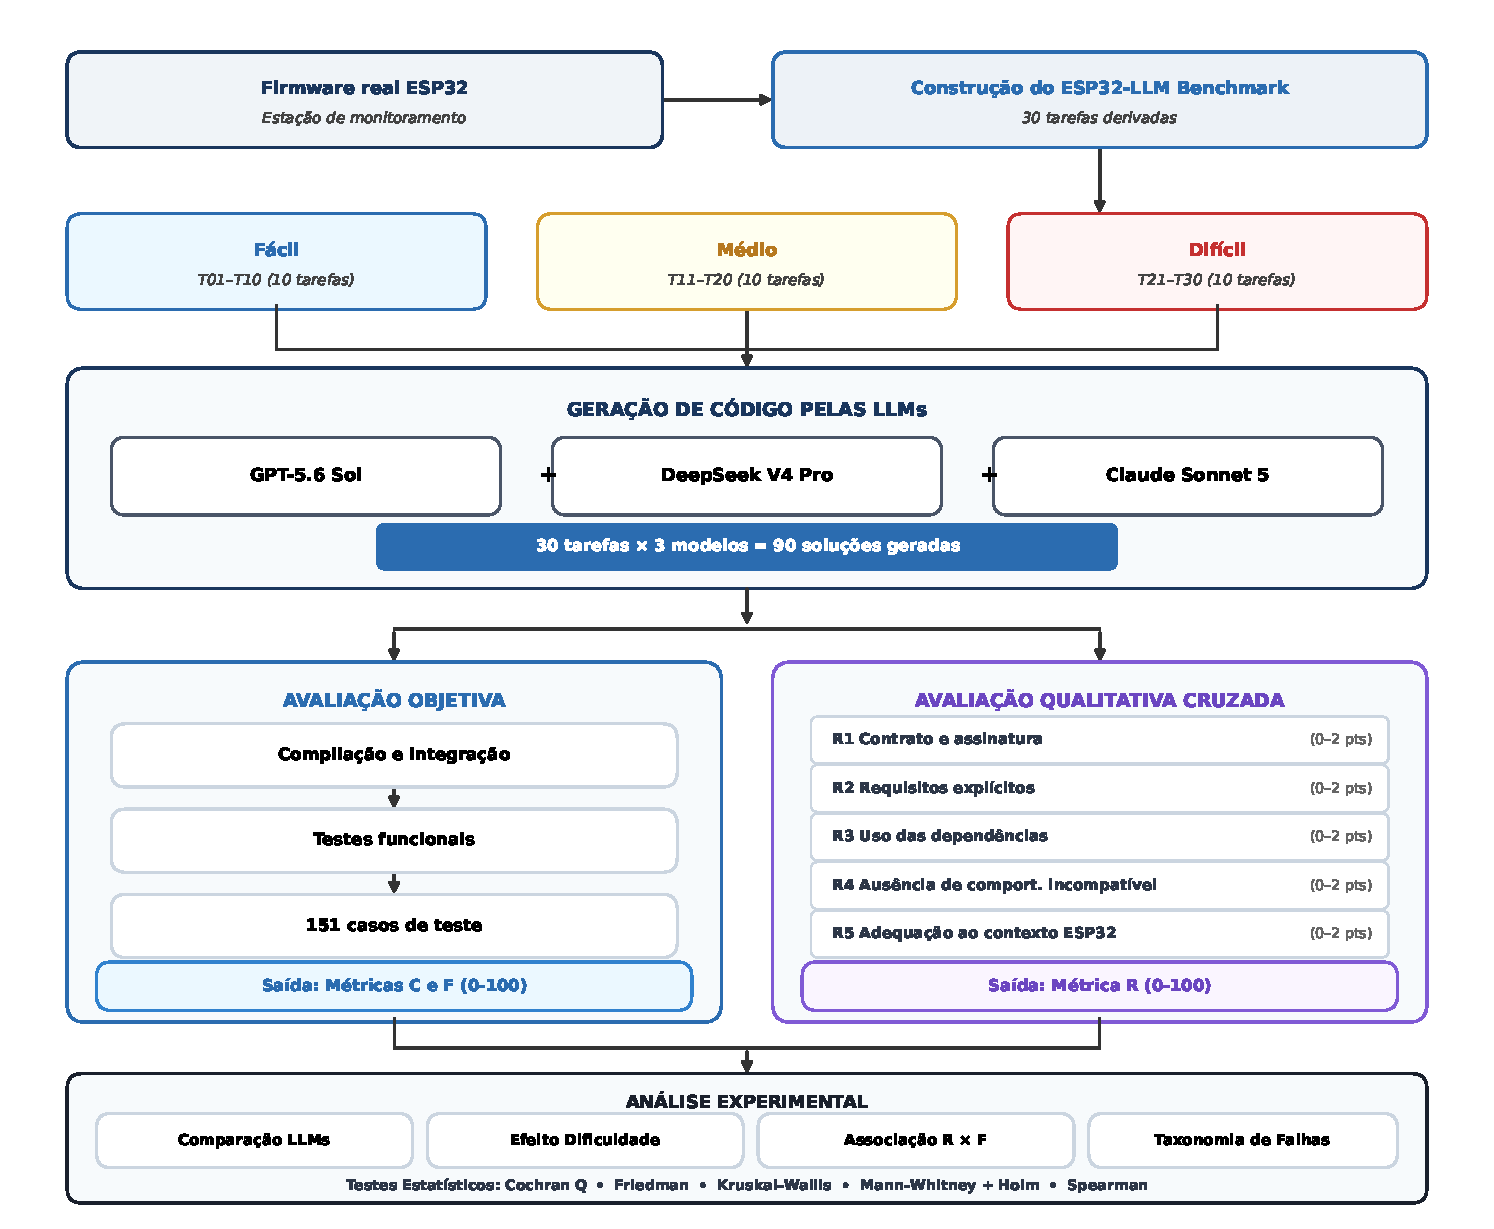
\includegraphics[width=\textwidth]{fluxo_metodologico_esp32_llm_sbc_compacto.pdf}
    \caption{Fluxo metodológico do ESP32-LLM Benchmark.}
    \label{fig:fluxo-metodologico}
\end{figure}



\subsection{ESP32-LLM Benchmark e LLMs}
\label{sec:benchmark}

O ESP32-LLM Benchmark foi construído a partir de um firmware real de uma estação de monitoramento baseada em ESP32, envolvendo aquisição de dados de sensores, cálculos, interrupções, EEPROM, serialização JSON, comunicação HTTP e serviços de configuração. Desse firmware foram derivadas 30 tarefas, cada uma submetida individualmente às LLMs por meio de uma especificação padronizada contendo contrato, contexto necessário e requisitos esperados. Os casos de teste foram definidos antes da geração das respostas.

As tarefas foram classificadas previamente em três grupos balanceados. As fáceis apresentam lógica predominantemente autocontida, interfaces simples e baixa dependência do restante do firmware. As médias envolvem periféricos, memória, interrupções ou estruturas específicas do sistema, mantendo escopo de integração delimitado. As difíceis apresentam maior dependência de estado global, bibliotecas, APIs e contratos de integração com diferentes componentes do firmware. A classificação não foi modificada após a obtenção dos resultados. A Tabela~\ref{tab:tarefas} apresenta as unidades experimentais.

\begin{table}[ht]
\centering
\caption{Tarefas que compõem o ESP32-LLM Benchmark.}
\label{tab:tarefas}
\small
\begin{tabular}{lll}
\hline
\textbf{Fácil} & \textbf{Médio} & \textbf{Difícil} \\
\hline
T01 -- passaTesteDegrau       & T11 -- isrPluviometro          & T21 -- setup \\
T02 -- Acumulador             & T12 -- isrAnemometro           & T22 -- loop \\
T03 -- detectarEeprom         & T13 -- identificarChipBmx      & T23 -- inicializarSensores \\
T04 -- lerUV                  & T14 -- lerPressaoAltitude      & T24 -- lerAmbiente \\
T05 -- faixaValida            & T15 -- lerLDR                  & T25 -- coletarAmostra \\
T06 -- calcularPontoOrvalho   & T16 -- calcularIndiceCalor     & T26 -- gravarRegistroPendente \\
T07 -- calcularITGU           & T17 -- escreverEEPROM          & T27 -- montarJSON \\
T08 -- calcularITU            & T18 -- lerEEPROM               & T28 -- enviarParaUmServidor \\
T09 -- classificarIndiceCalor & T19 -- calcularChecksum        & T29 -- tentarDrenarFila \\
T10 -- classificar            & T20 -- lerRegistro             & T30 -- configurarServidorAdmin \\
\hline
\end{tabular}
\end{table}

Foram avaliados GPT-5.6 Sol (LLM01), DeepSeek V4 Pro (LLM02) e Claude Sonnet 5 (LLM03), acessados pelas APIs dos respectivos provedores. O mesmo prompt de cada tarefa foi submetido aos três modelos, totalizando 90 soluções. Considerou-se apenas a primeira resposta, sem ciclos de correção, feedback dos testes ou refinamento iterativo, e nenhuma solução recebeu correção manual.

\subsection{Procedimento e Métricas de Avaliação}
\label{sec:procedimento}

A avaliação objetiva utilizou Arduino CLI 1.5.1, core \texttt{esp32:esp32} versão 3.3.8 e FQBN \texttt{esp32:esp32:esp32}. Cada solução foi integrada ao ambiente de teste da respectiva tarefa e compilada. As soluções compiláveis foram então submetidas aos casos funcionais previamente definidos. Dependências externas foram controladas pelos ambientes de teste e, nas tarefas dependentes de periféricos, utilizou-se uma configuração física padronizada do ESP32, mantendo o mesmo circuito e procedimento entre os modelos. Comparações de ponto flutuante utilizaram tolerâncias previamente definidas. O benchmark compreende 151 casos de teste.

Foram analisadas separadamente três dimensões, normalizadas entre 0 e 100: compilação e integração ($C$), desempenho funcional ($F$) e avaliação qualitativa ($R$). Para cada solução, $C=100$ indica compilação e integração bem-sucedidas, enquanto $C=0$ indica falha que impede a execução dos testes. Para soluções executáveis, $F$ corresponde à proporção de casos aprovados:
\begin{equation}
F = \frac{a}{n} \times 100,
\label{eq:funcional}
\end{equation}
em que $a$ representa o número de casos aprovados e $n$ o total de casos associado à tarefa. No cálculo do desempenho funcional no pipeline completo, soluções que não compilaram receberam $F=0$, pois não produziram comportamento executável passível de validação. Os resultados de $C$ são apresentados separadamente para distinguir falhas de compilação ou integração de falhas observadas nos testes funcionais.

A dimensão $R$ foi obtida por avaliação qualitativa cruzada, independentemente dos resultados de compilação e testes. Cada solução foi avaliada pelas duas LLMs que não a produziram, evitando autoavaliação. A rubrica compreendeu cinco critérios, pontuados de 0 a 2: preservação do contrato e assinatura (R1), atendimento aos requisitos explícitos (R2), uso coerente das dependências fornecidas (R3), ausência de comportamento incompatível (R4) e adequação ao contexto ESP32 e sistemas embarcados (R5). A soma, entre 0 e 10, foi normalizada para $R$ entre 0 e 100. Foram previstos 180 julgamentos, dos quais 177 foram utilizáveis; três julgamentos não retornaram conteúdo válido e foram tratados como ausentes. Casos com julgamento ausente ou diferença de pelo menos quatro pontos entre os avaliadores, na escala de 0 a 10, foram submetidos à auditoria humana empregando a mesma rubrica, totalizando quatro soluções auditadas. $R$ foi tratado como medida complementar e não agregado a $C$ ou $F$.

\subsection{Análise Estatística}
\label{sec:estatistica}

Como as mesmas 30 tarefas foram submetidas às três LLMs, as comparações entre modelos preservaram o pareamento por tarefa. Adotou-se $\alpha=0{,}05$. O sucesso de compilação foi comparado pelo teste $Q$ de Cochran e o desempenho funcional pelo teste de Friedman. Para avaliar o efeito da dificuldade, composta por conjuntos distintos de tarefas, aplicou-se Kruskal--Wallis separadamente a cada LLM, seguido, quando pertinente, por Mann--Whitney com correção de Holm e tamanho de efeito rank-biserial.

A associação entre $R$ e $F$ foi examinada pela correlação de Spearman no conjunto completo e separadamente por nível de dificuldade, permitindo verificar se uma associação global persistia após a estratificação. Resultados com $p<0{,}05$ foram considerados significativos; ausência de significância foi interpretada como insuficiência de evidência para rejeitar a hipótese nula, e não como demonstração de equivalência.

\section{Resultados}
\label{sec:resultados}

\subsection{Desempenho Geral e Efeito da Dificuldade}
\label{sec:desempenho-geral}

Considerando as 30 tarefas, o GPT-5.6 Sol apresentou $C=76{,}67$ e $F=76{,}67$, seguido pelo DeepSeek V4 Pro ($C=73{,}33$; $F=71{,}00$) e pelo Claude Sonnet 5 ($C=70{,}00$; $F=70{,}00$). Em números absolutos, compilaram 23 soluções do GPT, 22 do DeepSeek e 21 do Claude. Essas diferenças são descritivas, uma vez que os testes inferenciais apresentados na Seção~\ref{sec:resultados-estatisticos} não identificaram diferença estatisticamente significativa entre os modelos.

A Figura~\ref{fig:rcf-modelo-nivel} apresenta conjuntamente as métricas $R$, $C$ e $F$ por modelo e nível de dificuldade. Nas tarefas fáceis, os três modelos obtiveram $C=100$ e $F=100$. Nas médias, GPT-5.6 Sol e Claude Sonnet 5 mantiveram $C=100$ e $F=100$, enquanto o DeepSeek V4 Pro apresentou $C=100$ e $F=93$, devido a falhas funcionais parciais nas tarefas T13 ($F=80$) e T14 ($F=50$).

\begin{figure}[ht]
\centering
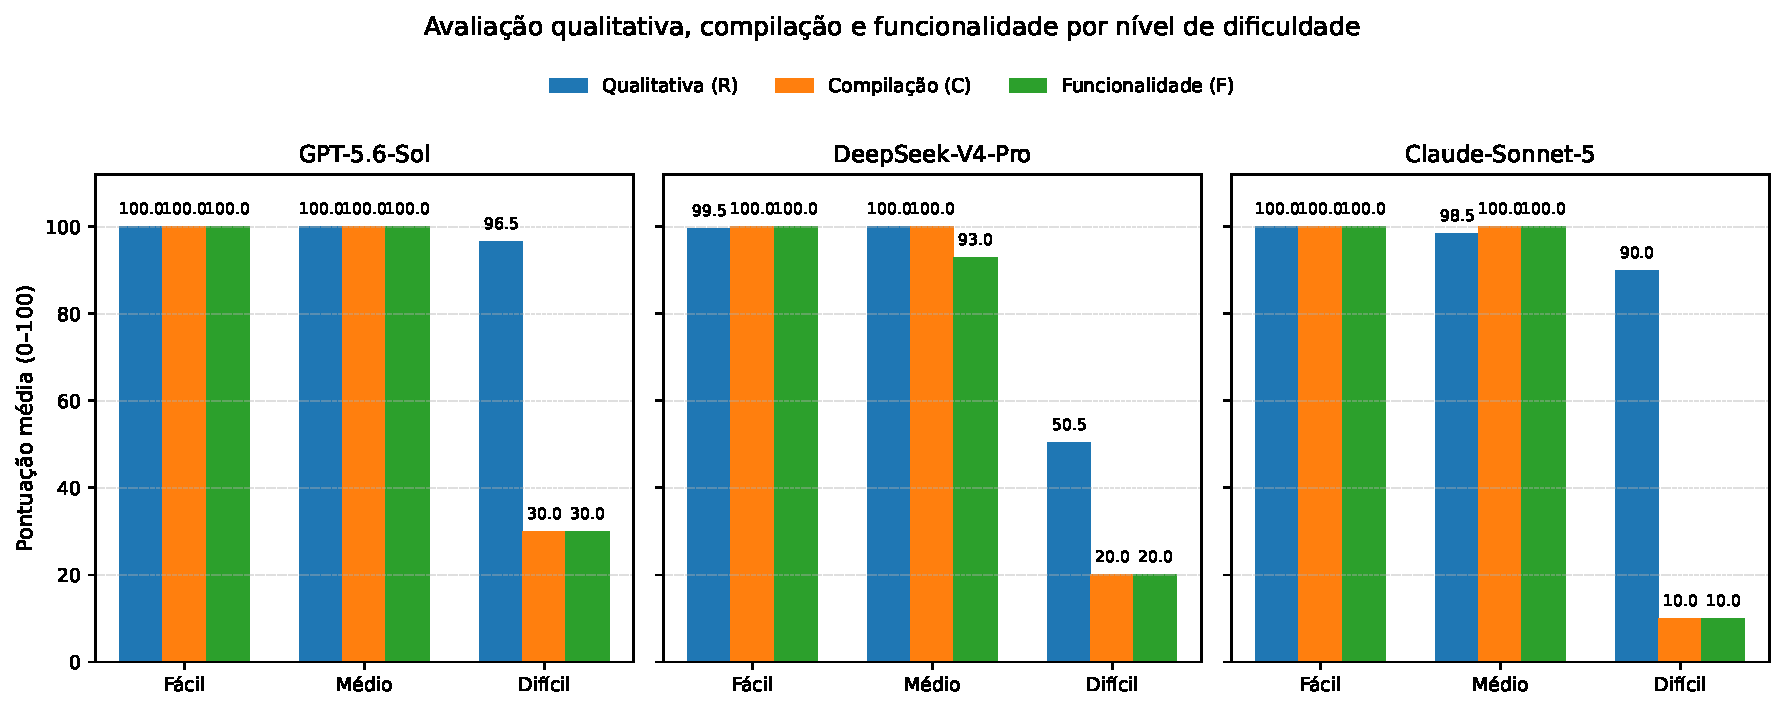
\includegraphics[width=0.98\columnwidth]{figura_01_R_C_F_por_modelo_nivel.pdf}
\caption{Médias de avaliação qualitativa ($R$), compilação ($C$) e correção funcional ($F$) por modelo e nível de dificuldade.}
\label{fig:rcf-modelo-nivel}
\end{figure}

A maior redução ocorreu nas tarefas difíceis: GPT-5.6 Sol apresentou $C=30$ e $F=30$, DeepSeek V4 Pro $C=20$ e $F=20$, e Claude Sonnet 5 $C=10$ e $F=10$. Das 30 combinações modelo--tarefa desse nível, apenas seis compilaram e foram aprovadas integralmente nos testes, enquanto 24 falharam na etapa de compilação ou integração. Não houve, nesse subconjunto, solução compilável com aprovação funcional apenas parcial, indicando que a redução de $F$ decorreu predominantemente de falhas anteriores à execução dos testes.

A Figura~\ref{fig:funcional-dificuldade} destaca a variação de $F$ entre os três níveis de dificuldade, evidenciando a queda de desempenho concentrada nas tarefas difíceis.

\begin{figure}[ht]
\centering
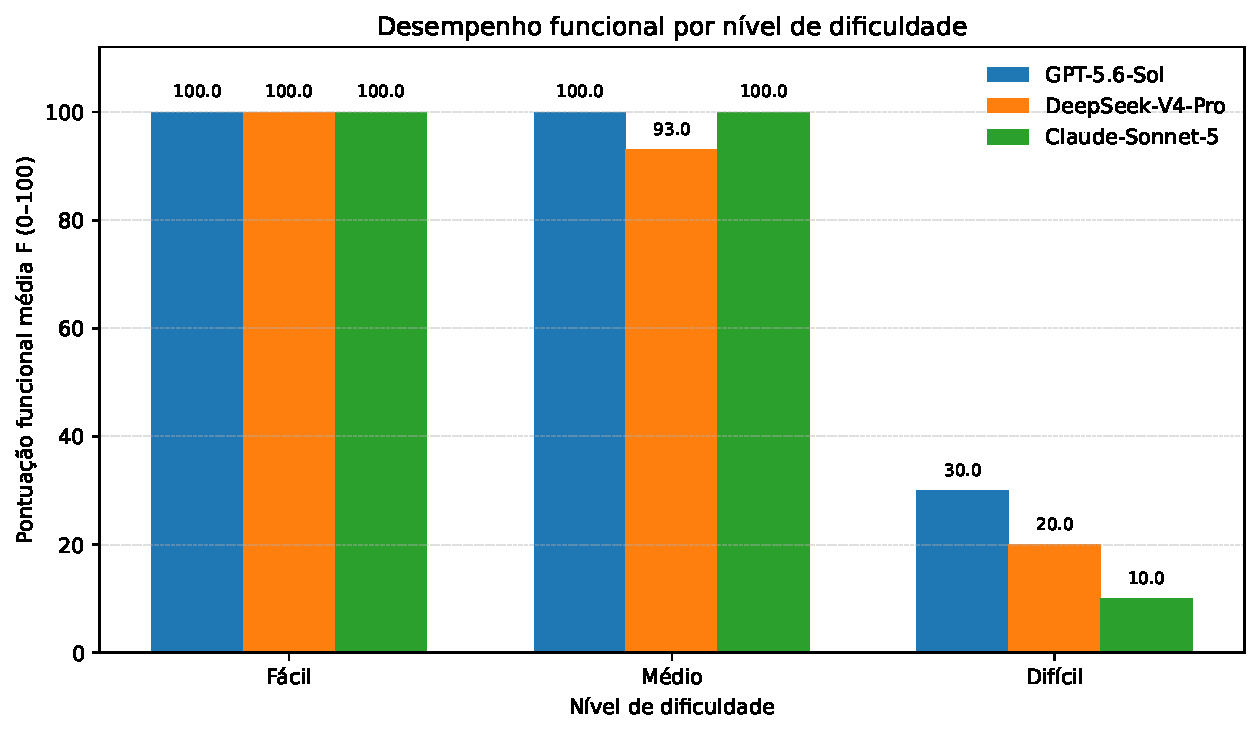
\includegraphics[width=0.90\columnwidth]{figura_02_funcionalidade_por_dificuldade.pdf}
\caption{Correção funcional ($F$) das LLMs nos três níveis de dificuldade.}
\label{fig:funcional-dificuldade}
\end{figure}

O sucesso nas tarefas difíceis concentrou-se em poucas unidades: T28 foi aprovada pelos três modelos, T22 pelo GPT-5.6 Sol e DeepSeek V4 Pro, e T21 apenas pelo GPT-5.6 Sol. As tarefas T23--T27, T29 e T30 não apresentaram sucesso objetivo para nenhum dos modelos.

\subsection{Análise Estatística}
\label{sec:resultados-estatisticos}

A comparação global entre as LLMs não revelou diferença estatisticamente significativa. Para compilação, o teste $Q$ de Cochran resultou em $Q=3{,}00$ e $p=0{,}223$; para correção funcional, o teste de Friedman produziu $\chi^2=3{,}50$ e $p=0{,}174$. Assim, não há evidência suficiente para estabelecer superioridade global de uma das LLMs neste experimento.

Em contraste, o efeito da dificuldade sobre $F$ foi significativo para GPT-5.6 Sol ($H=17{,}65$, $p<0{,}001$), DeepSeek V4 Pro ($H=17{,}64$, $p<0{,}001$) e Claude Sonnet 5 ($H=24{,}86$, $p<0{,}001$). Nas comparações par a par com correção de Holm, as diferenças fácil--difícil e médio--difícil permaneceram significativas: GPT ($p_{\mathrm{Holm}}=0{,}0032$ em ambas), DeepSeek ($p_{\mathrm{Holm}}=0{,}0013$ e $0{,}0033$) e Claude ($p_{\mathrm{Holm}}<0{,}001$ em ambas). A comparação fácil--médio do DeepSeek não foi significativa ($p_{\mathrm{Holm}}=0{,}168$).

Os tamanhos de efeito rank-biserial nas comparações com o nível difícil foram elevados: $0{,}70$ para GPT em ambas as comparações, $0{,}80$ e $0{,}76$ para DeepSeek e $0{,}90$ para Claude em ambas. Esses resultados corroboram que a principal variação de desempenho está associada às tarefas classificadas como difíceis.

\subsection{Falhas nas Tarefas Difíceis}
\label{sec:falhas}

Das 24 falhas de compilação ou integração observadas nas tarefas difíceis, 21 puderam ser classificadas conclusivamente. Dessas, 16 ($76{,}2\%$) corresponderam à incompatibilidade contextual (E3), envolvendo divergências em nomes, campos, estado compartilhado, constantes, tipos ou contratos esperados pelo firmware. Três ($14{,}3\%$) decorreram de implementação ausente ou incompleta (E2), e duas ($9{,}5\%$) do uso incompatível de APIs ou bibliotecas (E1). As três falhas restantes, referentes à T24, foram mantidas como indeterminadas e excluídas do cálculo das proporções.

\begin{figure}[ht]
\centering
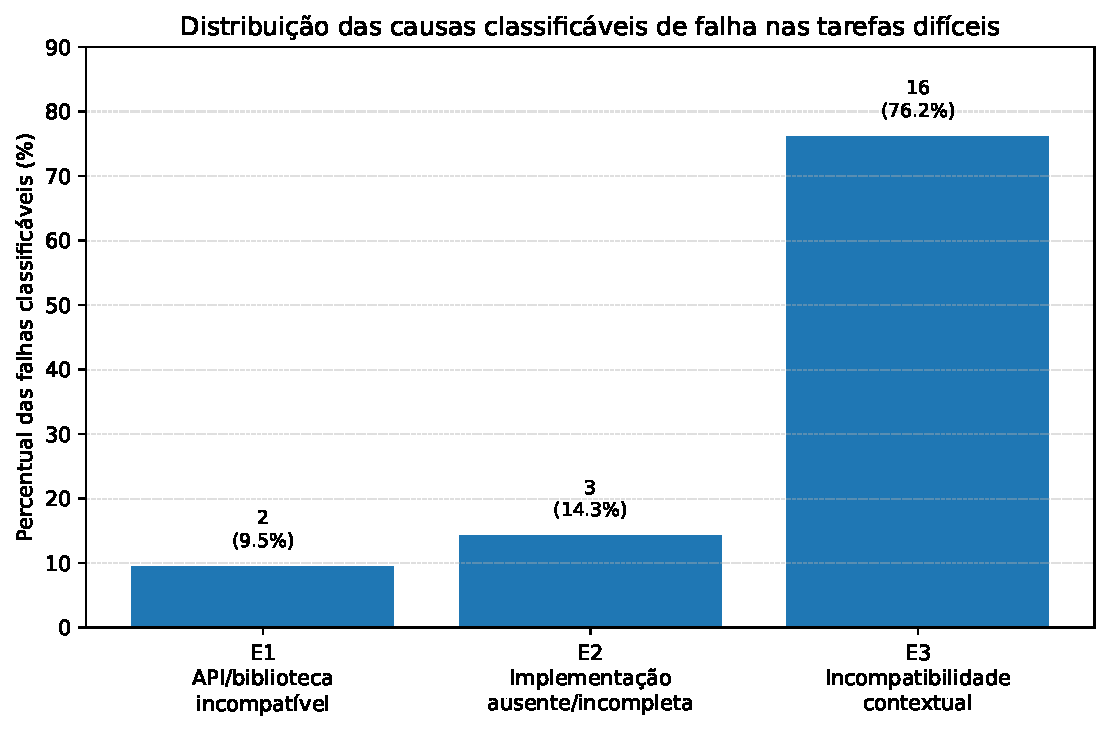
\includegraphics[width=0.88\columnwidth]{figura_04_taxonomia_falhas_dificeis.pdf}
\caption{Distribuição das categorias de falha entre as ocorrências classificáveis nas tarefas difíceis.}
\label{fig:taxonomia-falhas}
\end{figure}

O predomínio de E3 indica que, nas tarefas difíceis deste benchmark, a preservação dos contratos e dependências do firmware constituiu uma fonte de falha mais frequente do que problemas restritos à implementação local.

\subsection{Avaliação Qualitativa e Desempenho Objetivo}
\label{sec:qualitativa-objetiva}

A avaliação qualitativa ($R$) apresentou associação global positiva com o desempenho funcional ($F$), com correlação de Spearman $\rho=0{,}658$ ($p<0{,}001$, $N=90$). Entretanto, essa associação não se manteve quando os níveis de dificuldade foram analisados separadamente. Nas tarefas fáceis, $F$ foi constante em 100, impossibilitando uma correlação informativa; nas médias, $\rho=-0{,}050$ ($p=0{,}795$); e, nas difíceis, $\rho=0{,}292$ ($p=0{,}117$).

A divergência é particularmente evidente no nível difícil. O GPT-5.6 Sol apresentou $R=96{,}5$, mas $C=30$ e $F=30$; o Claude Sonnet 5 obteve $R=90{,}0$, com $C=10$ e $F=10$; e o DeepSeek V4 Pro apresentou $R=50{,}5$, com $C=20$ e $F=20$. Além disso, 18 soluções apresentaram $R\geq80$ e $F<100$, resultado utilizado apenas como análise descritiva exploratória.

Esses resultados indicam que a associação global entre $R$ e $F$ é influenciada pelas diferenças entre níveis de dificuldade e não fornece evidência de que uma avaliação qualitativa elevada, isoladamente, seja um indicador confiável de compilação e desempenho funcional.
```


\section{Discussão}
\label{sec:discussao}

Os resultados permitem responder às quatro questões de pesquisa. Em relação à RQ1, embora tenham sido observadas diferenças descritivas entre as LLMs, os testes estatísticos não forneceram evidência de superioridade global de um modelo quanto à compilação e à correção funcional. Da mesma forma, a ausência de significância estatística não deve ser interpretada como evidência de equivalência entre os modelos.

Quanto à RQ2, a dificuldade das tarefas apresentou efeito significativo sobre o desempenho das três LLMs, com a principal redução concentrada no nível difícil. Nesse nível, as falhas ocorreram predominantemente antes da execução dos testes funcionais, durante a compilação ou integração. Esse comportamento sugere que o aumento da dependência de hardware, APIs, estado compartilhado e contratos do firmware constitui um desafio relevante para a geração de código embarcado, em concordância com observações de Babiuch e Smutny~\cite{babiuch2026benchmarking}.

Para a RQ3, embora tenha sido observada associação global positiva entre avaliação qualitativa e desempenho funcional, essa relação não se manteve quando os níveis de dificuldade foram examinados separadamente. Nas tarefas difíceis, soluções qualitativamente bem avaliadas também apresentaram falhas de compilação ou integração. Assim, a inspeção qualitativa e as evidências executáveis capturam propriedades distintas, e avaliações favoráveis da estrutura e adequação aparente do código não substituem sua validação no ambiente-alvo.

Em resposta à RQ4, a incompatibilidade contextual foi a causa predominante entre as falhas classificáveis nas tarefas difíceis, envolvendo elementos como contratos, nomes, campos, tipos, constantes e estado compartilhado. Esse resultado indica que, em tarefas fortemente dependentes do sistema, produzir uma implementação local plausível não é suficiente: a solução também deve preservar as interfaces e dependências necessárias à integração com o firmware.

Em conjunto, os resultados indicam que benchmarks para geração de código em sistemas embarcados devem considerar tarefas com dependências reais de firmware, além de funções autocontidas. A combinação de compilação, integração, testes funcionais e inspeção qualitativa permite identificar falhas que poderiam permanecer ocultas em avaliações baseadas apenas na aparência ou estrutura do código.

\section{Limitações e Ameaças à Validade}
\label{sec:ameacas}

Quanto à validade externa, o benchmark foi derivado de um único firmware ESP32 e avaliou três LLMs em versões específicas, limitando a generalização para outros modelos, plataformas e domínios. Por outro lado, o uso de tarefas derivadas de firmware real permite avaliar dependências e contratos de integração pouco representados por problemas algorítmicos autocontidos.

Quanto à validade de construção, compilação e integração ($C$), desempenho funcional ($F$) e avaliação qualitativa ($R$) representam dimensões distintas. Soluções que não compilaram receberam $F=0$ por não produzirem comportamento executável, enquanto $C$ é apresentado separadamente para distinguir essas ocorrências. Possíveis vieses na avaliação qualitativa foram mitigados por avaliação cruzada sem autoavaliação, rubrica padronizada e auditoria humana nos casos ausentes ou com elevada discordância.

Quanto à validade interna, os casos de teste foram definidos previamente, os mesmos prompts e ambientes foram utilizados entre os modelos e as respostas foram preservadas sem correção manual. Na T27, identificou-se a ausência da dependência ArduinoJson; após a instalação da versão 6.21.6, a avaliação foi repetida para os três modelos, sem alteração das respostas, e as falhas persistiram. Os resultados oficiais correspondem à execução corrigida.

Na T24, uma execução posterior não reproduziu integralmente as falhas de compilação registradas no conjunto consolidado. Como os artefatos preservados não permitiram reconstruir inequivocamente as condições dos resultados oficiais, as três ocorrências foram mantidas como indeterminadas na taxonomia e excluídas do cálculo das proporções, evitando atribuir causas não sustentadas pelas evidências.

Por fim, foi considerada uma única geração por modelo e tarefa, sem refinamento ou feedback de compilação. Esse desenho controla a comparação e avalia a primeira resposta produzida, mas não representa cenários iterativos nos quais erros podem ser corrigidos após feedback do ambiente.

\section{Conclusão}
\label{sec:conclusao}

Este trabalho apresentou o ESP32-LLM Benchmark, uma abordagem experimental para avaliar a confiabilidade de código gerado por LLMs em tarefas derivadas de um firmware ESP32 real. A avaliação combinou compilação e integração, testes funcionais, análise qualitativa cruzada e métodos estatísticos, permitindo examinar diferentes dimensões da qualidade das soluções produzidas.

Os resultados mostraram desempenho elevado nas tarefas fáceis e médias e queda acentuada nas tarefas difíceis, com efeito estatisticamente significativo da dificuldade para as três LLMs avaliadas. Nas tarefas de maior complexidade, as falhas ocorreram predominantemente na compilação ou integração, sendo a incompatibilidade contextual a principal causa entre as ocorrências classificáveis. Além disso, soluções com avaliações qualitativas elevadas apresentaram, em alguns casos, baixo desempenho objetivo, indicando que a inspeção qualitativa isolada não é suficiente para determinar a confiabilidade do código gerado.

Esses achados reforçam a importância de avaliar código gerado por LLMs no contexto real em que será integrado, considerando dependências, contratos de software e evidências executáveis. Como trabalhos futuros, pretende-se ampliar o benchmark para diferentes firmwares e plataformas embarcadas, incorporar novas LLMs e investigar estratégias de geração iterativa, recuperação de contexto e feedback de compilação para reduzir falhas em tarefas com maior dependência do sistema.



\bibliographystyle{sbc}
\bibliography{sbc-template}

\end{document}


